\section{File Hash Threat Intelligence}
\label{sec:hash-analysis}

File hashes in a threat intelligence feed are indicators for malicious
files. It is one of the most lightweight ways to mark files as
suspicious. One can incorporate this data to block malicious
downloads, malicious email attachments, and malware. Likewise, file
hashes can be used to whitelist applications and these feeds can be
used to ensure malicious files do not appear in a customer's
whitelist. In this section we present our analysis on
eight file hash feeds, also collected from December 1st, 2017
to July 20th, 2018. We use the same metrics defined in
Section~\ref{sec:metrics}.

The file hash feeds we collected use a range of different hash
functions to specify malicious files, including MD5, SHA1, SHA256 and
SHA512 (and some feeds provided values for multiple different hash
functions to support interoperability).  Since most indicators in our
dataset are MD5s, we have normalized to this representation by using other
feeds and the VirusTotal service to identify hash aliases for known
malicious files (i.e., which MD5 corresponds to a particualr SHA256
value).  

I showed the detail result of the hash feeds analysis in 
Table~\ref{tab:md5-volume-1} and Table~\ref{tab:md5-volume-2}. The second column group presents feed 
volume, average daily rate, the number of converted MD5s 
(Section~\ref{sec:hash-overlap}) and exclusive proportion.
\textit{Not in VT} is fraction of hashes that are not found in 
VirusTotal, \textit{Not det.} the fraction of hashes that are found
in VirusTotal but are not labeled as malicious by any products, and
\textit{Detected} the fraction that are found in VirusTotal and are
labeled malicious by at least one product. Column \textit{Not in
SD} shows the fraction of hashes in a feed that are not in
Shadowserver Bin Check. \textit{In NSRL} and \textit{In AppInfo}
show the absolute number of hashes found in Shadowserver
(Section~\ref{sec:hash-accuracy}). \textit{Exclusive} is based on
the MD5-normalized hashes counted under \textit{Converted}. All the
other percentages in the table are based on \textit{Volume}. I
will explain about these result in detail in the followin sections.


\begin{table*}[htt]
\footnotesize \tabcolsep=0.11cm
\caption{File hash feeds overview (Part I)}
\centering
\small
\begin{tabular}{l | r r r r H H H H H H }
\toprule
 Feed         &   Volume  &  Avg. Rate  & Converted &   Exclusive  &   Not in VT    &  Not det.  &   Detected   &   Not in SD &   In NSRL   &  In AppInfo  \\
\midrule
 FB Malware              &    944,257  &  4,070    & 944,257   &    >99.99\%    &     37.41\%    &    50.50\%      &     12.09\%          &    99.89\% &     442 &             706 \\
 PA Malware Indicators   &    39,702   &  171      & 39,702    &     98.73\%    &      0.02\%    &     0.04\%      &     99.94\%          &   >99.99\% &       2 &             0  \\
 PA Analyst              &    38,586   &  166      & 37,665    &     97.97\%    &      4.26\%    &     2.82\%      &     92.92\%          &    99.95\% &       8 &             19 \\
 PA Twitter Emotet       &    1,031    &  4.44     & 960       &     77.29\%    &     11.74\%    &     0.78\%      &     87.49\%          &    99.81\% &       0 &             2  \\
 PA OSINT                &    829      &  3.57     & 783       &     71.65\%    &     19.06\%    &     0.84\%      &     80.10\%          &    99.88\% &       1 &             0  \\
 PA Sandbox              &    298      &  1.28     & 115       &     95.65\%    &     72.81\%    &     0.34\%      &     26.85\%          &    100\% &         0 &             0  \\
 PA Abuse.ch             &    267      &  1.15     & 3         &       100\%    &     98.88\%    &     0.75\%      &      0.37\%          &    100\% &         0 &             0  \\
 PA Zeus Tracker         &    17       &  0.07     & 17        &       100\%    &     88.24\%    &     5.88\%      &      5.88\%          &    100\% &         0 &             0  \\
\bottomrule
\end{tabular}
\label{tab:md5-volume-1}
\end{table*}


\begin{table*}[htt]
\footnotesize \tabcolsep=0.11cm
\caption{File hash feeds overview (Part II)}
\centering
\small
\begin{tabular}{l H H H H | r r r | r r r }
\toprule
 Feed         &   Volume  &  Avg. Rate  & Converted &   Exclusive  &   Not in VT    &  Not det.  &   Detected   &   Not in SD &   In NSRL   &  In AppInfo  \\
\midrule
 FB Malware              &    944,257  &  4,070    & 944,257   &    >99.99\%    &     37.41\%    &    50.50\%      &     12.09\%          &    99.89\% &     442 &             706 \\
 PA Malware Indicators   &    39,702   &  171      & 39,702    &     98.73\%    &      0.02\%    &     0.04\%      &     99.94\%          &   >99.99\% &       2 &             0  \\
 PA Analyst              &    38,586   &  166      & 37,665    &     97.97\%    &      4.26\%    &     2.82\%      &     92.92\%          &    99.95\% &       8 &             19 \\
 PA Twitter Emotet       &    1,031    &  4.44     & 960       &     77.29\%    &     11.74\%    &     0.78\%      &     87.49\%          &    99.81\% &       0 &             2  \\
 PA OSINT                &    829      &  3.57     & 783       &     71.65\%    &     19.06\%    &     0.84\%      &     80.10\%          &    99.88\% &       1 &             0  \\
 PA Sandbox              &    298      &  1.28     & 115       &     95.65\%    &     72.81\%    &     0.34\%      &     26.85\%          &    100\% &         0 &             0  \\
 PA Abuse.ch             &    267      &  1.15     & 3         &       100\%    &     98.88\%    &     0.75\%      &      0.37\%          &    100\% &         0 &             0  \\
 PA Zeus Tracker         &    17       &  0.07     & 17        &       100\%    &     88.24\%    &     5.88\%      &      5.88\%          &    100\% &         0 &             0  \\
\bottomrule
\end{tabular}
\label{tab:md5-volume-2}
\end{table*}

\subsection{Volume}

File hashes, unlike IP threat data, are not transient---a file does
not change from malicious to benign---and thus a far simpler volume
analysis is appropriate. I report volume as the number of new hashes
that are added to each feed during the measurement period.

As seen in Table~\ref{tab:md5-volume-1}, I examine each feed's volume and
average daily rate. Like IP feeds, file hash feeds also vary dramatically in
volume. The majority of the hashes are concentrated in three feeds: FB Malware,
PA Malware Indicators, and PA Analyst, which also exhibit the highest daily rates.
The other feeds are multiple order of magnitude smaller comparatively.

%Every feed has mostly exclusive content, with the ``lowest'' exclusivity belonging to PA Twitter Emotet and PA OSINT (still 77.6\% and 79.29\%, respectively). All other feeds showcase a >97\% exclusive percentage, demonstrating that most MD5 feeds are distinct from each other.

\subsection{Intersection and Exclusive Contribution}
\label{sec:hash-overlap}

As we mentioned earlier, to conduct intersection and exclusive
analysis of file hash feeds, we need to convert indicators into the
same hash type. Here we convert non-MD5 hashes into MD5s, using either
metadata in the indicator itself (i.e., if it reports values for
multiple hash functions) or by querying the source hash from
VirusTotal~\cite{VirusTotal} which reports the full suite of hashes
for all files in its dataset.  However, for a small fraction of hashes
we are unable to find aliases to conver them to the MD5 representation
and must exclude them from the analysis in this section.  This filtering is
reflected in Table~\ref{tab:md5-volume}, in which the Volume column
represents the number of unique hashes found in each feed and the Converted
column is the subset that we have been able to normalize to a MD5
representation.

\finding\ The intersections between hash feeds are minimal,
even among the feeds that have multiple orders of magnitude differences in size.
Across all feeds, only PA Analyst has relatively high intersections: PA Analyst
shares 27\% of PA OSINT's MD5s and 13\% of PA Twitter Emotet's MD5s. PA Malware
Indicators has a small intersection also with these two feeds. All other
intersections are around or less than 1\%. Consequently, the vast majority of
MD5s are unique to one feed, as recorded in column \textit{Exclusive} in
Table~\ref{tab:md5-volume}. The ``lowest'' exclusivity belongs to PA Twitter
Emotet and PA OSINT (still 77.29\% and 71.65\%, respectively). All other feeds
showcase an over 95\% exclusive percentage, demonstrating that most file hash feeds
are distinct from each other.

Due to the different sources of malware between feeds, a low intersection is to
be expected in some cases. For example, PA Twitter Emotet and PA Zeus Tracker
should have no intersection, since they are tracking different malware strains.
The other, more general feeds could expect some overlap, but mostly exhibit
little to no intersection. Considering the sheer volume of the FB Malware feed,
one might expect it would encapsulate many of the smaller feeds or at least
parts of them. This is not the case, however, as FB Malware has a negligible
intersection with all other feeds.

Due to the lack of intersection among the feeds, we omit the latency analysis
of the hash feeds, as there is simply not enough intersecting data to conclude
which feeds perform better with regards to latency.

%\subsection{Latency}
\label{sec:hash-timing}
\note{We might need to delete this section since the overlapped parts are too small, we can't make an argument about latency}

We use the same relative latency definition to calculate the latency distribution of MD5s in each feed, and the calculation is based on the shared data between feeds. Since MD5s are not transient, we don't need to set a time restriction for this computation. Figure~\ref{fig:md5-latency} shows the latency distribution CDF of the feeds.

\begin{figure}[h]
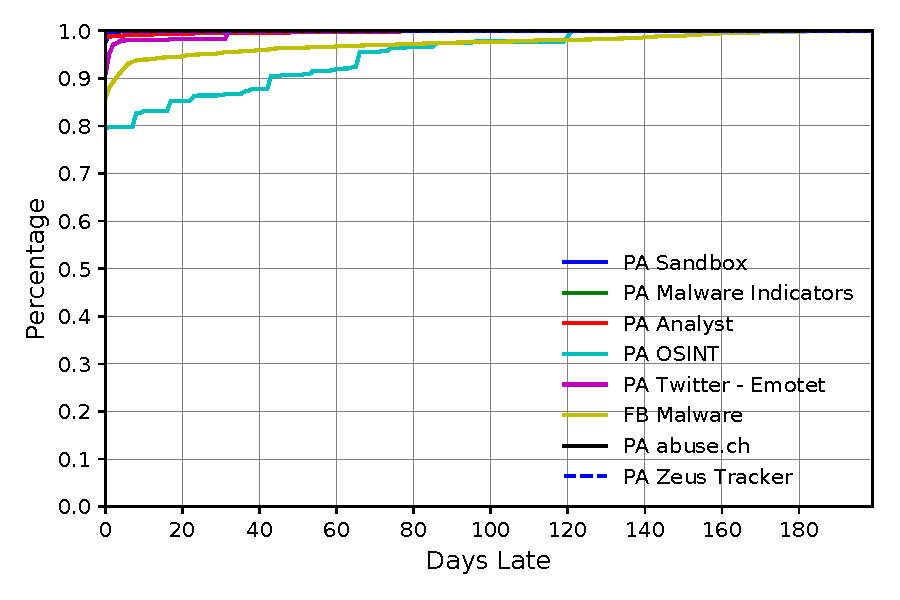
\includegraphics[width=0.9\columnwidth]{images/md5_lateDay.pdf}
\caption{Feed Latency Distribution showing what percentage of each feed's intersected samples are on a particular delay.}
\label{fig:md5-latency}
\end{figure}

As seen in Figure~\ref{fig:md5-latency}, the feeds are roughly grouped into 3 areas. {PA Malware Indicators}, {PA Zeus Tracker}, {PA Analyst}, {PA Twitter - Emotet}, {PA abuse.ch} and {PA Sandbox} report over 90\% of their data first, while {FB Malware }reports over 85\% of its data first. PA OSINT is the outlier in the graph which reports only 80\% of its shared data first. It also has the largest delays, taking almost 50 days to reach 90th percentile and over 70 days to reach 95th percentile.

\finding\ The latency analysis shows which feed is more effective from a timing standpoint, and again demonstrates the fact that a large \ti\ source is not always the quickest at reporting threats.

\subsection{Accuracy}
\label{sec:hash-accuracy}
Assessing the accuracy of file hash feeds presents a problem: there is no
universal ground truth to determine if a file is malicious or benign. Thus,
to gauge the accuracy of the feeds, we use two metrics: a check for malicious
hashes against VirusTotal, and a check for benign hashes against Shadowserver's
Bin Check service. Note that all the percentages discussed below are based on
the \textit{Volume} of each feed.

\subsubsection{VirusTotal}

VirusTotal is a service that is often used when analyzing
malware to get a base of information about a suspected file.
Anyone can upload a file to be scanned. Upon submission, these files will be
scanned by more than 70 antivirus scanners, which creates a report on how many
antivirus scanners mark it malicious, among other information. In this analysis,
we query VirusTotal for the hashes in each file hash feed and then inspect the
percent of hashes that are marked as malicious and how many AV scanners have
recorded them. Due to the high volume of the FB Malware feed and the query
rate limit of VirusTotal, we randomly sampled 80,000 hashes from the feed for
this analysis.

Table~\ref{tab:md5-volume} shows a breakdown of the base detection rates for
each feed from VirusTotal. As the PA feeds decrease in volume, the rates at
which they are found in VirusTotal also decreases. The larger PA feeds have a
much higher detection rate than their smaller counterparts. On the other hand,
FB Malware only has 37\% of its data detected by antivirus scanners and 50\% in
VirusTotal with no detection despite being the largest feed. This could indicate
that FB Malware focuses on threats that specifically target Facebook and that
are not as relevant to most VirusTotal users, such as malicious browser
extensions~\cite{dekoven2017malicious, jagpal2015trends, kapravelos2014hulk}.
This might undermine the limited coverage of VirusTotal as an oracle to detect
targeted threats that are not of broader interest.

\begin{figure}[t]
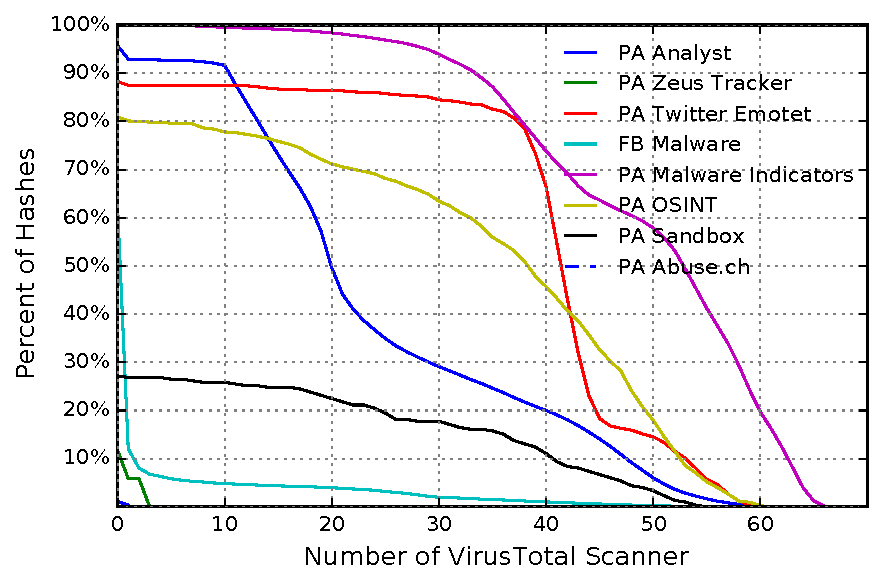
\includegraphics[width=0.95\columnwidth]{images/hash_vt_cdf.pdf}
\caption{VirusTotal detection distribution. Each point means the proportion of indicators (Y value) in a feed that is detected by \textit{over} X number of AV scanners in VirusTotal.}
\label{fig:vt-cdf}
\end{figure}

To further understand how the scanners in VirusTotal report the feed's data,
we plot a graph of what percentage of hashes in each feed are detected by how many
VirusTotal scanners. As seen in Figure~\ref{fig:vt-cdf}, four feeds have more
than 50\% of their samples detected by over 20 scanners. PA Malware Indicators
and PA Twitter Emotet did not experience a large detection drop before 35 scanners,
indicating that most indicators in the two feeds are popular malicious files
recognized by many AV vendors. While PA Sandbox has a large percent of its hashes
not presented in VirusTotal, over 70\% of its samples that are detected are marked
by over 20 AV scanners, showcasing a high confidence detection.

\subsubsection{Shadowserver}

To more fully gauge the accuracy of the file hash feeds,
we also examined how each feed measured against Shadowserver's Bin Check
Service~\cite{shadowserver}. The service checks file hashes against NIST's
National Software Registry List (NSRL) in addition to Shadowserver's own repository of
known software. Table~\ref{tab:md5-volume} details how each feed compares with
Shadowserver's Bin Check service.

It might be expected that there would be no hash found with Shadowserver's Bin
Check service, but it is not the case. Some of the samples from the feeds that
appear in Shadowserver are well known binaries such as versions of Microsoft
Office products, Window's Service Packs, calc.exe, etc. In the event malware
injects itself into a running process, it remains plausible that some of these
well-known binaries find their way into \ti\ feeds from users wrongly attributing
maliciousness. While FB Malware has over one thousand hashes in Shadowserver, this
is not a widespread issue, as all feeds have <1\% of their hashes contained within
Shadowserver's Bin Check service.
%, shown in Table \ref{tab:md5-volume}.
This showcases that while there are a few exceptions, the feeds mostly do not
contain well-known, benign files.

\finding\ Each PA feed has a negligible rate of occurrence within Shadowserver
regardless of their VirusTotal detection, showing they do not contain generic
false positives. Larger feeds exhibit high VirusTotal detection rates except
for FB Malware, while small feeds have relatively low detection rates.
This suggests that small hash feeds might focus more on specific malicious files
that are not widely known.
FB Malware has a low VirusTotal occurrence despite
its size and has over one thousand hashes in Shadowserver, but its overall low
percentage of hashes within Shadowserver indicates that it does not contain
many known files and might have threats not typically recognized by
VirusTotal's scanners.

